\documentclass[12pt]{article}

\title{Data Analysis Project Report}
\author{James Hughes}

\usepackage[nottoc,numbib]{tocbibind}
\usepackage{graphicx}

\newcommand\NA{\mathit{NA}}

\begin{document}

\begin{titlepage}
    \begin{center}
        \vspace*{1cm}

        \Huge
        \textbf{Structured Illumination Microscopy Image Processing using Deep Learning}

        \vspace{0.5cm}
        \LARGE

        James Hughes

        Supervised by Dr Edward Ward

        \vspace{2cm}
        \Huge
        \textbf{Project Report}

        \vfill

        MPhil, Data Intensive Science

        \vspace{0.8cm}

        \Large
        Department of Physics \& Department of Chemical Engineering and Biotechnology

        University of Cambridge

        United Kingdom

        28th June 2024

    \end{center}
\end{titlepage}

\pagenumbering{roman}

\newpage
\section*{Acknowledgements}
\addcontentsline{toc}{section}{\protect\numberline{}Acknowledgements}

Firstly I would like to thank my supervisor, Dr Edward Ward, for all of his support over the course of this project.
The project involved a lot of concepts from microscopy and image processing that were very new to me,
but Dr Ward made it clear from early on in the project that this would not be a problem,
and was quick to provide reading materials to help me get to grips with the subject.
Having been trained in mathematics during my time as an undergraduate,
the chance to go into the laboratory and capture real microscope images that were later used in the work was incredibly exciting.
Dr Ward was eager to provide this opportunity and welcomed me to the Chemical Engineering and Biotechnology (CEB) Department and his research group.

I also had the opportunity to attend some of the Laser Analytics Group (LAG) lab meetings,
where I had the privilege of learning about some of the world-leading research being undertaken by the group.
Later, I shared details about my own project in two presentations to the group.
I would like to thank all of the members of the LAG for welcoming me, listening to my presentations and providing great feedback.
In particular I wish to thank Professor Clemens Kaminski for his helpful suggestions and words of encouragement.

I would also like to thank Jeremy Wilkinson, Esther Gray, and Emilio Luz-Ricca.
I had very insightful conversations about the project with all of them that helped me see the work in a new light.

Lastly, I would like to thank my parents for being a continual source of support and strength throughout my education,
in particular for encouraging me to make the most of every opportunity that comes my way.

\newpage
\begin{abstract}
    \addcontentsline{toc}{section}{\protect\numberline{}Abstract}

    Structured illumination microscopy (SIM) produces images whose resolution exceeds the Abbe diffraction limit imposed on widefield images.
    However, SIM imaging of dynamic cellular processes is restricted by phototoxicity effects, which limit the maximum duration of such time-lapses.
    In 2023, Li et al. developed a `two-step denoising' approach to SIM image processing,
    which enables greatly reducing the illumination intensity of the microscope,
    and in turn using deep learning to recover the lost signal in the image.
    Firstly, this project presents a data processing pipeline which implements their method using PyTorch.
    This pipeline is documented, modular, and open-source, enabling researchers to apply the method to different datasets, or develop extensions to the work.
    Secondly, this project investigates the reproducibility of this method, by analysing its performance on two datasets:
    microtubule images acquired using a 2D SIM microscope and
    synthetic 3D SIM imagery simulated by using data from the Visible Human Project as ground-truth.
    Results indicate that although the first-step reconstructions can improve the fidelity compared to the low SNR inputs,
    this is potentially dependent on the variety of the biological structures present in the training data.
    Moreover, while the performance of the full two-step denoising method produces images qualitatively close to ground-truth,
    with noticeably reduced reconstruction artefacts compared to the raw and first-step reconstructions,
    there is little quantitative evidence that the second step increases image fidelity,
    calling into question the reliability of this second network.


\end{abstract}

\newpage
\tableofcontents

\newpage
\pagenumbering{arabic}
\section{Introduction}

Fluorescence microscopy is an essential tool for microbiologists,
enabling them to view complex biological phenomena unfolding at the sub-cellular level.
Fluorescent dyes are employed to attach to specific organic compounds,
which then release photons in response to illumination from a laser at a suitable wavelength,
producing images that highlight specific structures of interest to researchers.
As a type of optical microscopy, the resolution of these systems is limited by the effects of diffraction.
This limit was quantified by Abbe \cite{abbe} in 1873 as a minimal resolvable distance between two points,

\[d=\frac{\lambda}{2\NA}\]

where $\lambda$ refers to the emittance wavelength, and $\NA$ refers to the numerical aperture,
a property of the optical system and the imaging medium.
This resolution limit is summarised by the optical transfer function $O(\vec{k})$ of the microscope,
which describes the set of spatial frequencies of the sample structure that can be captured by the optical system,
and to what extent they are attenuated in the resulting image (in frequency space).
Axial resolution of optical microscopes is typically much worse than their lateral resolution.
This fact is evidenced by the optical transfer function's omission of most k-vectors that lie along and near to the z-axis,
a phenomenon referred to as the `missing-cone problem'.
This is further compounded in practice with issues such as spherical abberation.
This represents a serious obstacle to researchers attempting to view cell dynamics in greater detail.

Structured Illumination Microscopy (SIM) is a technique that combines a specialised microscope set-up,
alongside computational processing of the acquired images,
in order to surpass the classical Abbe diffraction limit.
The theoretical foundations of the technique were first established in 2008 \cite{originalSIM},
but since then there have been a range of improvements made to the technique [citations].
While SIM does not necessarily provide the greatest improvements in resolution compared to other methods such as confocal,
it has other advantages for researchers interested specifically in capturing imagery of dynamic biological processes over extended periods.
This relates primarily to the issue of phototoxicity effects.
Every time a fluorescence microscopy image of a cell sample is taken, the cell itself is bleached and damaged in the process.
This is particularly troublesome when one wishes to view dynamic processes in live cells,
because the very process of imaging has an effect on the process being captured,
thereby limiting the duration of imagery that can be obtained that is faithful to the true process.
SIM offers a trade-off between resolution improvements and low photo-toxicity effects.

The paper by Li et al. \cite{keypaper} explores augmenting the SIM image processing pipeline with deep-learning techniques to improve this trade-off.
Their research explores multiple ways in which hardware and computation can be used to improve the resolution of SIM imaging.
This project investigates their `two-step denoising method'.
In this method, the illumination intensity of the SIM system is set to around 10 times lower than usual,
in order to mitigate phototoxicity effects.
In turn, they train two networks to denoise the acquired and reconstructed images,
in order to compensate for the noise introduce by the low illumination dose and reclaim lost image resolution.

This project aims to present a full pipeline that implements their method.
The tools developed in the repository aim to make this software accessible to other research groups looking to apply it to their own data,
with minimal work required for set-up, and compatibility with common tools used for SIM image processing.
Moreover, by adopting an open-source ethos, this project should enable the pipeline to be extended upon easily.
The second main objective of this work is to study the reproducibility of the results claimed in the original research.
In particular, Li et al. assert that this method:
\begin{itemize}
    \item mitigates the presence of artefacts in the reconstructions of low SNR acquisitions,
    \item improves the resolution of SIM imaging, particularly the axial resolution, and,
    \item increases the fidelity of reconstructed images by up to 3.63dB (PSNR) on average.
\end{itemize}
This work sets out to apply the method to both microtubule data collected from a 2D SIM system,
as well as synthetically generated 3D SIM data, and compare the resulting reconstructions.

\section{Methods}

\subsection{SIM Reconstruction process}


Structured Illumination Microscopy stands in contrast to the conventional approach of using a uniform illumination to produce a micrograph image.
Instead, SIM microscopes usually employ a spatial light modulator (SLM) to produce a striped illumination pattern,
whose spacing is close to the Abbe diffraction limit of resolution.
When the light illuminates the sample causing it to fluoresce,
the excitation pattern's spatial frequencies interfere with the high spatial frequencies of the structures in the sample,
causing information to be exposed as lower frequency features in the resulting image \cite{originalSIM}.
Figure \ref{fig:moire} demonstrates this effect with Moir\'{e} fringes,
an interference pattern with lower spatial frequency than the two patterns that generate it.

\begin{figure}[hbt]
    
\includegraphics[scale=0.5]{figures/moire.png}
    \caption{Moir\'{e} Fringes}
    \label{fig:moire}
\end{figure}

In order to correctly interpret this interference effect, and reconstruct a super-resolved image,
multiple images need to be acquired from the microscope and analysed in the Fourier domain \cite{originalSIM}.
When reconstructed properly, there will be an improvement of lateral resolution in the direction of the k-vector of the pattern.
Therefore, when acquiring images for 2D SIM, it is almost always 3 groups of images that are acquired,
using patterns whose orientations are angled at multiples of $2\pi/3$ radians,
to obtain an near-isotropic improvement in \textit{lateral} resolution,
and the same is true in 3D SIM.
Within these groups, the images are acquired with the illumination pattern having a different phase each time,
typically with a constant offset between phases.

The reconstruction involves six key steps:

\begin{enumerate}
    \item parameter estimation,
    \item fourier transform,
    \item band separation,
    \item Wiener filtering,
    \item apodization, and,
    \item inverse Fourier transform.
\end{enumerate}

Parameter estimation is primarily concerned with the position of the illumination pattern,
including the phase, angle, and modulation depth.
This is more accurate than measuring these quantities in the physical system which would require high degree of care and precision.
Then the image is converted to the frequency domain.

Denoting the image intensity by $D(\vec{r})$, the pattern k-vector and phase by $\vec{p}$, $\phi_n$,
the modulation depth by $a_m$, the density of the fluorescent substance as $S(\vec{r})$ and the point-spread function by $H(\vec{r})$,
we see that the effect of the optical system on the `true' ground-truth structure $S$ is to multiply it with the excitation pattern,
and then convolve with the point-spread function:

\[D_n(\vec{r}) = \sum_{m=-M}^{M}{S(\vec{r})a_m\exp(im(2\pi\vec{p}\cdot\vec{r}+\phi_n))\otimes H(\vec{r})}\]

Utilising the Convolution Theorem this becomes

\[\tilde{D}_n(\vec{k}) = \sum_{m=-M}^{M}{\exp(im\phi_n)a_m\tilde{S}(\vec{k}-m\vec{p})\tilde{O}(\vec{k})}\]

In turn, with sufficient acquired images at different phases, namely M, this can be used to solve a fully determined set of linear equations for

\[\tilde{S}(\vec{k}-m\vec{p})\tilde{O}(\vec{k})\qquad m=-M,\dots,M-1,M\]

This constitutes the band separation step, and explains why 2D SIM uses 3 sets of 3 images, while 3D SIM uses 3 sets of 5 images;
the number of different phases used in imaging must correspond to the number of delta peaks that represent the illumination pattern in Fourier space,
in order to set up a fully-determined system of linear equations \cite{params}.

The steps of Wiener filtering and apodization are used to combine the separated bands of the image, ...

The parameters used for the reconstructions are shown in Table \ref{tab:reconparams}

\begin{table}[htp]
    \centering
    \begin{tabular}{| c | c | c | c |}
        \hline
        Parameter & 2D Dataset (1) & 2D Dataset (2) & 3D Dataset \\
        \hline
        $\NA$  & 1.1 & 1.1 & 1.12 \\
        \hline
        Pixel width (nm) & 107 & 107 & 50 \\
        \hline
        Wavelength (nm) & 488 & 561 & 464 \\
        \hline
        OTF param.  & 0.15 & 0.15 & 0.15 \\
        \hline
        APO cutoff & 1.59 & 1.68 & 1.82 \\
        \hline
        APO bend  & 1.0 & 1.0 & 1.0 \\
        \hline
        Wiener parameter & 0.05 & 0.05 & 0.05 \\
        \hline
        RL Iterations & 5 & 5 & 5\\
        \hline

    \end{tabular}
    \caption{Parameters used to reconstruct the images in fairSIM.}
    \label{tab:reconparams}
\end{table}

\subsection{Data}

In the original work, Li et al. acquired pairs of high and low SNR images from a 3D SIM system,
in order to train the networks.
This project takes a slightly different approach,
simulating the increased image noise from a lower the illumination intensity in-silico.
This makes the acquisition of the training data much faster,
and avoids the need for image-pair registration, along with the errors that this could induce.
A low SNR image is simulated from the ground-truth high SNR image on a pixel-by-pixel basis:
a pixel whose value is $N$ in the high SNR image is set to a random draw of a Poisson random variable whose rate parameter is $N$/$s$,
where $s$ is some chosen scale factor constant across all pixels and images.
In both datasets this scale factor is set as 20.

The method is applied to a dataset of 2D SIM images in the first instance,
in which the fluorescent dye marks microtubules within the cells.
This contains more high spatial frequency content that can be resolved by SIM than an earlier dataset acquired for the project,
in which viruses and the cell membrane of the host cell were highlighted.
The samples were illuminated with visible light at 488nm and 561nm.

In the second case, the Visible Human Dataset\footnote{Courtesy of the U.S. National Library of Medicine} is used to generate synthetically acquired 3DSIM micrographs.
This dataset was released in 1994 [cite] and provides images of human cadavers prepared as a series of thousands of thin cross sections.
The work uses the 70mm photographs of the female body dataset, image 2000 through to 2383.
While this imagery does not capture \textit{microscopic} biological structures,
those biological structures present are complex enough to yield an approximation to the image features one might expect from a typical SIM micrograph of a cell.
These images are downloaded, cropped into 256x256 squares 3 and stacked into image volumes of size (128, 256, 256).
Figure \ref{fig:vhcrop} shows the lateral cropping scheme overlayed onto image 2192,
the central image slice used.
The cropping is designed to produce 60 image volumes that mostly overlap with the biological subject matter,
for a total of 180 volumes when all 384 images are processed.

\begin{figure}[hbt]
    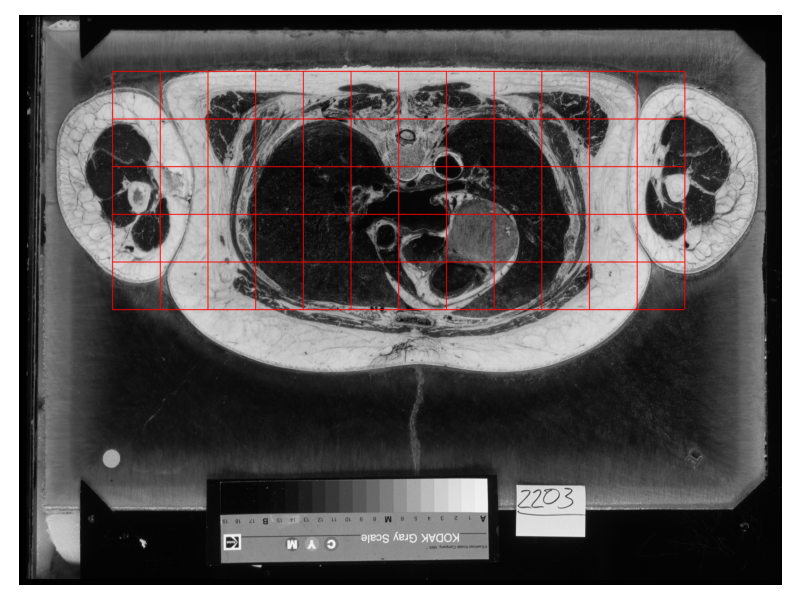
\includegraphics[scale=0.65]{figures/visible_human_volumes_grey.png}
    \caption{Cropping of Visible Human Dataset images}
    \label{fig:vhcrop}
\end{figure}

The volumes are then processed using \texttt{generate\_sim.py} to generate synthetic SIM acquisitions.
This script was adapted from [cite].
Originally, this script took an image volume of size (64, 256, 256) and generated an image stack of size (15, 256, 256),
simulating 15 SIM acquisitions from a microscope whose focal plane is at the central (32nd) slice of the 3D volume.
This was adapted further to simulate a 3D SIM microscope with a vertically moving objective lens and focal plane.
This effect was achieved by cropping the bottom $n$ lateral slices of the 3D volume and padding the top of the volume with $n$ zero-filled layers,
in order to move the focal plane to z-slice $32-n$ of the original volume.
A loop was used to generate a full (32, 15, 256, 256) 3DSIM acquisition stack,
equivalent to imaging the top half of the sample.
Each of the image volumes generated with a height of 128 voxels was used to generate two of these stacks.

[Diagram]

Splitting up of data.

\subsection{Pipeline}

Migration to TensorFlow

The first step of the data processing pipeline is to produce the training-validaition-testing partition,
which can be done using \texttt{image\_noising.py}.
This script takes a directory of high-SNR images, produces the synthetic low-SNR data counterpart images,
and then splits the data into training, validation, and testing partitions randomly.
In this work, 20\% of each dataset was reserved as testing data,
and a further 20\% of the remaining images were reserved for validation at the end of each epoch.

An RCAN model is then trained using this partitioned data - the 'first-step' model.
This step is handled by the \texttt{train.py} script.
The code first reads in the configuration for training from a JSON file.
This file specifies:
\begin{itemize}
    \item training hyperparameters; such as number of epochs and the learning rate,
    \item model hyperparameters, and,
    \item file management; including the frequency of model checkpointing and the locations of training and validation data.
\end{itemize}
Configuring the hyperparameters in this way ensures that it is easier to keep track of the many training runs that may be performed.
Next, the training and validation data is read one file at a time, to perform checks---for instance to ensure that all of the images are of the same shape,
and that the data is consistent with model hyperparameters.
After this, the relevant training objects are instantiated: the model itself, the Adam optimizer, and the learning rate scheduler.
If an intermediate model checkpoint has been provided, all of these objects are updated to match the state of this checkpoint,
to enable continued training.
Alongside these is the \texttt{SIM\_Dataset} object wrapped in a \texttt{torch.utils.data.DataLoader} which handles the batching of training (and validation) data.

During training, this dataset object handles generation of suitable ground-truth and raw data.
Crucially, the RCAN input shape is smaller than the images themselves,
so the \texttt{SIM\_Dataset} takes random matching crops of the training pairs that correspond to the RCAN input shape.
It then normalises the pixel values, using an affine rescaling to map extreme image-wide pixel value percentiles to 0 and 1;
this work uses the values 2\% and 99.9\% respectively.
Before these crops are outputted, they are also subjected to a random 90 degree rotation about the z-axis,
and two random reflections in the lateral axes.
This data augmentation increases the number of possible output crops by 16-fold,
on top of the number of possible crop locations.
Accordingly, the dataset object takes a \texttt{steps\_per\_epoch} parameter---this
parameter controls exactly how many times each image in the dataset is exposed to the training loop per epoch,
but with various different transformations.
In addition, the object is also able to filter for regions of interest.
The number of pixel values (scaled in the $[0, 1]$ range) that exceed some intensity threshold can be counted,
and then crops with an insufficient fraction of pixel values above this level can be excluded.
However, this slows down the speed of batch-loading, not just because of the rejection rate,
but also the computation required to run this check.

The model is then applied to the raw images.

Preprocessing of all images

Reconstruction (for 3D, CZXY->PAZ) including stacking and destacking

Postprocessed

Step 2 training (post processed as well, althoguh this doesnt have an effect?)

Software best practices
I/O, documentation, modularity, version control

Using CSD3, hardware, parallel -> serial

\subsection{RCAN}

In both instances, the denoising models were implemented using the residual channel attention network (RCAN) architecture,
which first emerged in the computer vision literature in 2018 \cite{rcan2018}.

Li et al. employed a slight variant of the RCAN implemented more recently \cite{rcan2021}.
In particular, this variant is re-implemented as a denoising model rather than a super-resolution model,
so there is no upsampling of the images over the course of the network architecture.
However, the code provided alongside this more recent work is written in TensorFlow.
In order to make the code compatible with the software available (specifically the versions of CUDA and cuDNN available) on the HPC platform used,
this codebase was migrated to PyTorch.
This also has the advantage of making the software more accessible to other researchers wishing to develop in PyTorch.

\section{Results}

Affine rescaling to minimize the MSE to the GT?
Discuss the results they found

\subsection{2D Data}

Parameter estimation

Generalizability

Tables of results, metrics

Images

SIM check results!

\subsection{3D Data}

Axial resolution

Tables of results, metrics

Images

\section{Discussion}
Results/conclusions
Further work
What I learned
How I could have improved
    - Augmentation: randomly permute the acquisitions?

\bibliographystyle{IEEEtran}
\bibliography{Biblio}

\appendix

\section{Statement on the use of auto-generation tools}

\section {High-Performance Computing Resources}

This work was performed using resources provided by the Cambridge Service for Data Driven Discovery (CSD3) operated by the University of Cambridge Research Computing Service (www.csd3.cam.ac.uk),
provided by Dell EMC and Intel using Tier-2 funding from the Engineering and Physical Sciences Research Council (capital grant EP/T022159/1),
and DiRAC funding from the Science and Technology Facilities Council (www.dirac.ac.uk).

\end{document}
